% update/discussion.tex -- interpretation and design-analysis material moved
% out of the Experiments section, which had grown to twelve subsections.
\section{Discussion}
\label{sec:discussion}

\subsection{Which mechanism is doing the work}
\label{sec:mechanism_shift}

The speedups above are produced by three mechanisms acting together: sizing the
hardware, reducing bytes through the precision, sparsity and memory-technology
decisions, and amortizing the reload through speculation. Because each is a
separate certified design in our formulation, we can decompose the result rather
than attribute it: we solve the same program with the mechanisms enabled
cumulatively, under one search configuration, and read off what each contributes.
\Cref{tab:mechanism} reports the decomposition, and its totals agree with
\cref{tab:batch} to within $0.02\times$ at every batch.

The dominant mechanism is not fixed; it shifts with the serving regime. At
single-stream decoding, hardware sizing carries $55\%$ of the gain and
speculation only $20\%$: the reload is small, so provisioning compute and
bandwidth is what buys speed. By $B=128$ this has inverted, with hardware
carrying $7\%$ and speculation $68\%$. The byte-reduction decisions are the steady middle
throughout, between $25\%$ and $34\%$. This is the same physics as the widening
of $K^\star$, seen from the other side: a larger batch gives each verification
pass a larger reload to amortize, so the amortizing mechanism displaces the
provisioning one. It also explains an observation in \cref{tab:perftdp} that is
otherwise surprising, namely that a single chip configuration
($24.4\times$ MACs, $3200$~GB/s, $422$~W) is selected at $B=8$, $32$ and $128$
alike: beyond low batch, additional silicon is not what buys the speedup.

The methodological consequence matters more than the individual percentages. A
sequential pipeline that fixes the hardware first and then schedules onto it
commits to a provisioning decision before knowing which mechanism the regime
will reward, and would over-provision silicon at high batch while
under-speculating everywhere. Deciding all three jointly is what allows the
program to move the weight between them as the regime changes, and the
decomposition here is the direct evidence that the weight does move.

\begin{table}[h]
\centering
\footnotesize
\caption{Cumulative certified stages and each mechanism's share of the total
gain above $1\times$, under one search configuration. Each stage is a separately
certified achievable design, so the shares decompose solved results rather than
estimating an attribution.}
\label{tab:mechanism}
\begin{tabular}{@{}rrrrrrrr@{}}
\toprule
& \multicolumn{3}{c}{Cumulative speedup} & & \multicolumn{3}{c}{Share of total gain} \\
\cmidrule(lr){2-4}\cmidrule(lr){6-8}
$B$ & hardware & $+$ decisions & $+$ spec.\ $K^\star$ & $K^\star$ &
hardware & decisions & speculation \\
\midrule
$1$   & $18.68\times$ & $26.55\times$ & $33.13\times$ & $2$  & $\mathbf{55.0\%}$ & $24.5\%$ & $20.5\%$ \\
$8$   & $6.67\times$  & $18.91\times$ & $36.76\times$ & $8$  & $15.9\%$ & $34.2\%$ & $49.9\%$ \\
$32$  & $4.73\times$  & $16.49\times$ & $44.85\times$ & $16$ & $8.5\%$  & $26.8\%$ & $\mathbf{64.7\%}$ \\
$128$ & $4.32\times$  & $16.06\times$ & $48.64\times$ & $32$ & $7.0\%$  & $24.7\%$ & $\mathbf{68.4\%}$ \\
\bottomrule
\end{tabular}
\end{table}


\subsection{Dual variables show what actually binds}
\label{sec:binding}

A certified optimum carries more information than its objective value. The dual
variable on each constraint is the rate at which the objective would improve if
that constraint were relaxed, and by complementary slackness a constraint with a
zero dual is not limiting the design at all. Reading them tells us what the
program is really up against, and the answer is unambiguous.

At the selected design the dual on the speculative verification pass is $129$.
The dual on the area cap is $8.7\times10^{-5}$, on the decode-traffic rows
$7.1\times10^{-5}$, and on the mixture-of-experts residency knapsack
$1.2\times10^{-5}$. The duals on the \emph{power cap} and on the \emph{pin-count
cap} are both exactly zero. The verification pass, which is to say the decode
memory wall, dominates every physical cap on the chip by roughly six orders of
magnitude. These designs are limited by the traffic they must move, not by the
silicon, the package or the power budget available to move it.

Two consequences follow, and we state them because each is easy to get wrong.
First, a cap can be nearly saturated without binding. The pin cap admits
$3277$~GB/s and the selected design runs at $3200$~GB/s, so it sits at $97.7\%$
of the limit; nevertheless its dual is zero, because the constraint's effect is
to remove the wider bandwidth branches from the menu rather than to be tight at
the chosen one. High utilization of a resource and scarcity of that resource are
different statements, and only the dual distinguishes them.

Second, this predicts which modelling refinements can matter. Any change that
relieves a zero-dual constraint cannot move the optimum, whatever its
physical merit. When we refined the program to charge a precision-dependent
compute energy (\cref{sec:energy_coeff}), a correction we regard as necessary
for the model to be right, the certified designs did not move at all, at either
end of the batch range. That is not a null result to be explained away; it is
what complementary slackness requires, and it was predictable from the dual
vector before the experiment was run. The same reasoning tells us that a
clock-clock-gating decision would be inert here for the same reason, which is why we do
not introduce one. The decisions that move these designs are the ones that reduce
decode traffic, and the duals say so before any of them is tried.

\subsection{Solving the Large Scale Systems Problem}
\label{app:custom_solve}
One of the central challenges in co-design optimization as noted in prior work~\citep{zhang_fast} is the limitations of existing solvers in handling the simultaneous extreme large scale and extreme ill-conditioned LPs inherent in the systems setting. At LLM scale the raw constraint matrix mixes unit-magnitude selection rows with execution rows whose coefficients reach $10^{10}$ cycles: a coefficient dynamic range of ${\sim}10$ orders of magnitude, and hence an effective conditioning of $\kappa \gtrsim 10^{10}$ that unscaled first-order methods cannot absorb (Section~\ref{sec:solver_vm}).
The joint tiling, fusion, placement, and rematerialization LP model for Llama-3 70B and DeepSeek-V3 has roughly 1.6\,M--2.5\,M decision variables, 1.9\,M--3\,M
constraints, and 4\,M nonzeros at minimum. Discretization of $L \approx 720$--$903$ layers, $C = 16$--$20$ pareto tile configs,
and $T = L$ timesteps yield more performant fine-grained optimization, but also presents increasingly challenging problem formulations for solvers to find convergent solutions. 
At this structure and scale, simplex and barrier solvers exhaust factorization memory, since traditional solvers were not engineered to refactor sparse Jacobians of this shape.
% The variable layout is
% \[
%     T[L] \;\mid\; y[L,C] \;\mid\; p[E,T] \;\mid\; p_W[L,T]
%     \;\mid\; r[L,T] \;\mid\; w[L,C,3] \;\mid\; h_{\mathrm{GM}}[K],
% \]
% for $L \approx 720$--$903$ layers, $C = 16$--$20$ Pareto tile configs,
% and $T = L$ timesteps. At this scale, simplex and barrier solvers exhaust
% factorization memory, and traditional solvers were never engineered to
% refactor sparse Jacobians of this shape.

\paragraph{CHEETAH LP Structure.} Extreme matrix ill-conditioning in the systems modeling setting is unavoidable. Timeloop per-tile cycle counts $T_{\min}(c)$ and $T_{\max}(c)$ span $10^3$--$10^{10}$ cycles.
The McCormick-envelope variables inject products of these
tile counts with normalized residency variables, so absolute matrix
entries span ${\sim}10^7$ in magnitude. The row-norm ratio exceeds well past $10^6$, and practically exceeds what generic interior-point methods can tolerate without diverging. 
However, this combination of scale $\times$ conditioning $\times$ solve speed
indicates a regime where first-order methods of the 
primal-dual hybrid gradient family (PDHG; \cite{chambolle2011first}) is the most feasible and credible path.
PDHG eliminates matrix factorization entirely, costs $\mathcal{O}(\text{nnz})$
per step, and converges as long as the operator can be preconditioned and
step sizes chosen suitably and adaptively. 

\paragraph{Custom solver design.}
We implement a custom variant of the PDHG solver in JAX. 
This is necessary since a custom built pre-conditioner and scaling regime is needed to successfully solve the ill-conditioned systems LP to convergence. This also helps reduce the co-design iteration time from days to hours. 
PDHG is dominated by sparse matvecs and elementwise projection operations that vectorize cleanly under XLA. 
Our custom solver implementation utilizes JAX's Just in Time (JIT) compilation and \texttt{lax.scan} over the inner iteration to batch ${\sim}10^5$ iterations onto the GPU/TPU at a few microseconds each. This also enables JIT-fusion of the Ruiz preconditioning~\citep{ruiz2001scaling} loop into a single kernel.

Naive JAX implementation of the PDHG solver for LPs~\citep{applegate2026pdlp} does not converge on CHEETAH systems LPs. 
This is unsurprising since first-order methods frequently cause the duality gap to oscillate and the standard symmetric-restart heuristic kept overshooting on our ill-conditioned problems. 
To solve this, we introduce a custom variable-metric one-sided rescue method (\textbf{VM-One-Armed-Rescue}) to produce convergence.
This novel asymmetric, one-sided method incorporates Halpern-reflection~\citep{halpern1967fixed} restarts in PDHG with a diagonal variable metric especially designed for CHEETAH-V1's large-scale systems LP structure. 
Additional solver design details are described in Appendix~\ref{append::lp_perform}.
This enables the primal and dual convergence of the systems LPs within ${\sim}80$--$200$\,s at feasibility tolerance $2.5\times10^{-7}$, reaching within 0.1--1\% of
the mature HiGHS optimum (the rounding gap is bounded and reported in Appendix~\ref{app:solver}). 
In contrast, existing PDHG solvers and off-the-shelf HiGHS either time out,
factorize into NaNs, or polish to objectives $5$--$12\times$ worse
without achieving dual convergence. 
The primal and dual convergence of our custom systems solver is also what enables the dual variable signal in the LLM Architect outer loop (Section~\ref{sec:llm_outer}).



\subsection{CHEETAH Design Blueprint Discussion}
\label{app:blueprint_tables}
The pre-fusion memory stall is the modeled fraction of unfused execution
time spent waiting on DRAM before fusion, tensor pinning, and placement
reduce traffic. Formally, 
\[
\mathrm{stall}_{\mathrm{pre}}
=
\frac{T_{\mathrm{pre}}-T_{\mathrm{compute}}}{T_{\mathrm{pre}}},
\qquad
T_{\mathrm{pre}}
=
\max(T_{\mathrm{compute}},T_{\mathrm{DRAM,pre}}).
\]
Here \(T_{\mathrm{compute}}\) is the pure compute floor assuming operands
are available on chip, and \(T_{\mathrm{DRAM,pre}}\) is the DRAM service
time of the unfused schedule. Thus a pre-fusion stall of \(97.5\%\)
indicates that the unfused schedule is dominated by  DRAM memory-stalled, and
only \(2.5\%\) of the modeled pre-fusion wall time is practically useful compute.

We write \(\text{stall}_{\text{pre}}\) and \(\text{stall}_{\text{post}}\) to denote the memory-stall fractions before and after fusion, respectively. 
Fusion efficiency measures the fraction of avoidable pre-fusion memory
stall that fusion and placement can unblock:
\[
\mathrm{fusion\ efficiency}
=
\frac{
\mathrm{stall}_{\mathrm{pre}}-\mathrm{stall}_{\mathrm{post}}
}{
\mathrm{stall}_{\mathrm{pre}}
}.
\]
Therefore, the combination of \(97.5\%\) pre-fusion stall and
\(100.0\%\) LP fusion efficiency in \cref{tab:cheetah_two_blueprints}
signifies that the unfused schedule is largely DRAM memory-stalled, which
CHEETAH alleviates by finding a fused placement schedule for which the post-fusion
DRAM floor falls below the compute floor. This is validated in the
post-fusion roofline audit, where
\(T_{\mathrm{DRAM}}/T_{\mathrm{compute}}\ll1\), so the LP optimum is
compute-bound. This is one of CHEETAH's key advantages: by reducing the idle DRAM-wait time through optimized global buffer and unified co-design configurations to unlock aggressive fusion, raising overall operational intensity.
% \cref{tab:cheetah_two_blueprints} presents two custom example designs found by CHEETAH-V1, 
% optimized for the Llama-3 70B and DeepSeek-V3 workloads individually. Appendix~\ref{app:blueprints} presents comprehensive blueprints of designs for different workloads, processes and data types. 

% The pre-fusion memory stall is calculated as the fraction of execution time that would be spent waiting on DRAM before fusion, tensor pinning,
% placement to reduce traffic, and etc. Formally,
% \[
% \text{pre-fusion mem stall}
% = \frac{T_{\text{pre}}-T_{\text{compute}}}{T_{\text{pre}}}.
% \]

% Here \(T_{\text{compute}}\) denotes the modeled pure compute time of the workload, (i.e., the time spent performing arithmetic assuming the operands are available on-chip with no DRAM stalls). 
% \(T_{\text{pre}}\) denotes the modeled total pre-fusion runtime.
% \(T_{\text{DRAM,pre}}\) denotes the modeled DRAM service time before fusion, tensor pinning, and placement optimizations are applied. Therefore \(T_{\text{pre}}=\max(T_{\text{compute}},T_{\text{DRAM,pre}})\). 


% We write \(\text{stall}_{\text{pre}}\) and \(\text{stall}_{\text{post}}\) to denote the memory-stall fractions before and after fusion, respectively. 
% Fusion efficiency measures the fraction of avoidable pre-fusion memory
% stall that fusion and placement can unblock:
% \begin{equation}
%     \text{fusion efficiency}
%     = \frac{\text{stall}_{\text{pre}} - \text{stall}_{\text{post}}}
%            {\text{stall}_{\text{pre}}}.
%     \label{eq:fusion_efficiency}
% \end{equation}


% Therefore, the combined pre-fusion mem stall = 97.5\% and fusion efficiency = 100.0\% values of~\cref{tab:cheetah_two_blueprints} signify that before fusion the schedule is almost entirely DRAM memory-stalled, which CHEETAH's modeling framework eliminates. This is further validated by the fact that $T_{\text{DRAM}} / T_{\text{compute}} \ll 1$.
% This summarizes one of the key advantages CHEETAH unlocks. Since the individual workloads are heavily memory-stalled regimes on the naive TPUv3 baseline, CHEETAH's unified framework jointly optimizes global tradeoffs that places, pins, and fuses tensors aggressively such that the modeled operating point becomes compute-bound, with zero residual memory stall.
% This reduces the idle DRAM-wait time through optimized global buffer and unified co-design configurations to unlock aggressive fusion and raises overall operational intensity.
% These quantities are roofline-model diagnostics, not
% measured silicon utilization; real implementations would still incur
% NoC, SRAM, pipeline, and control overheads.
% \mnote{usually with DRAM you want burst sequential reads, not scattered random reads, you tell DRAM i want to read form this address for however many bytes of data, there's a whole bunch of cycles you have to wait before you get your first piece of data. }


\begin{table}[t]
\centering
\caption{
Two CHEETAH-V1 accelerator designs showing distinctly different regimes.
The Llama-3 70B design is an efficient and balanced variant,
contrasting the DeepSeek-V3 design which is the bandwidth-rich variant.
All designs presented pass the six pre-RTL
manufacturability gates roofline checks.
}
\label{tab:cheetah_two_blueprints}
\small
\setlength{\tabcolsep}{4pt}
\begin{tabular}{@{}lcc@{}}
\toprule
 & \textbf{CHEETAH-V1 Llama-3 70B} & \textbf{CHEETAH-V1 DeepSeek-V3} \\
 & \textbf{Efficient} & \textbf{Bandwidth-Rich} \\
\midrule
Process                        & TSMC N7                          & TSMC N5 \\
Memory system                       & LPDDR5X (8 packages)             & HBM3 (3 stacks) \\
Memory capacity                     & 128 GB                           & 72 GB \\
Memory peak BW                      & 544 GB/s                         & 2{,}457 GB/s \\
Die area                            & 425 mm$^2$                       & 485 mm$^2$ \\
TDP (compute + memory IO)           & 392 W                            & 434 W \\
Peak compute @ 1 GHz                & 3,539 TOPS (INT8)              & 2,621 TOPS (INT8) \\
PE grid                             & $48 \times 36 = 1,728$ PEs & $32 \times 40 = 1,280$ PEs \\
PE systolic array dims              & $32 \times 32$                   & $32 \times 32$ \\
PE vector width                     & 64 lanes                         & 64 lanes \\
PE L1 buffer size (in / wt / out)   & 16 / 16 / 16 KB                  & 16 / 16 / 16 KB \\
PE L1 config                        & Private                          & Private \\
PE L2 config                        & Shared                           & Shared \\
Global buffer size                  & 64 MiB                           & 64 MiB \\
\midrule
Pre-fusion mem stall               & 97.5\%                           & 97.2\% \\
Fusion efficiency                   & 100.0\%                          & 100.0\% \\
OpInt ridgepoint                    & 6{,}505 ops/byte                & 1{,}066 ops/byte \\
Fused model OpInt                   & $2.07 \times 10^{6}$ ops/byte   & $1.46 \times 10^{6}$ ops/byte \\
$T_{\text{DRAM}} / T_{\text{compute}}$ at actual BW & $3.14 \times 10^{-3}$ & $7.29 \times 10^{-4}$ \\
Binding constraint at LP optimum    & compute                          & compute \\
Achieved speedup vs.\ naive TPU-v3 & $\mathbf{40.16\times}$  & $\mathbf{35.68\times}$ \\
\midrule
LP Solver & \texttt{custom JAX PDHG} & \texttt{custom JAX PDHG} \\
LP Solve Time & 13.4 s & 21.1 s \\
\bottomrule
\end{tabular}
\end{table}
% \subsection{Simulator Validation}



% \subsubsection{LLM Architect vs. Optimizer}
% The LLM Architect framework is modeled on SkyDiscover, and efficiently prunes the large outer hardware search loop by proposing campaign patches. Rather than predicting performance, the Architect reads a compact Causal Ledger containing invalid-rate history, MFU, roofline lower-bound checks, and LP diagnostics, then proposes a constrained hardware neighborhood for Vizier to search locally. The V1 LP remains the sole performance evaluator: for each candidate, it solves the joint tiling, fusion, placement, and rematerialization LP, while a deterministic Roofline Auditor rejects physically impossible results. In the widened V1 search space, all methods reach the same capped V1 Perf/TDP ceiling, so the key differentiator is search efficiency. The LLM loop reduces invalid hardware evaluations from 24.5\% under full-space Vizier to 5.9\% on average across five workloads, a 4.1× reduction in wasted trials, while preserving the same best V1 score. This shows that the LLM’s contribution is not replacing Vizier or the solver, but steering Bayesian optimization toward feasible, workload-appropriate architectural neighborhoods with far less wasted trials. This also sets the foundation for future work, where the LLM in the loop can adhere to follow more complex human reasoning signals.
% \begin{figure}[ht!]
%     \centering
% 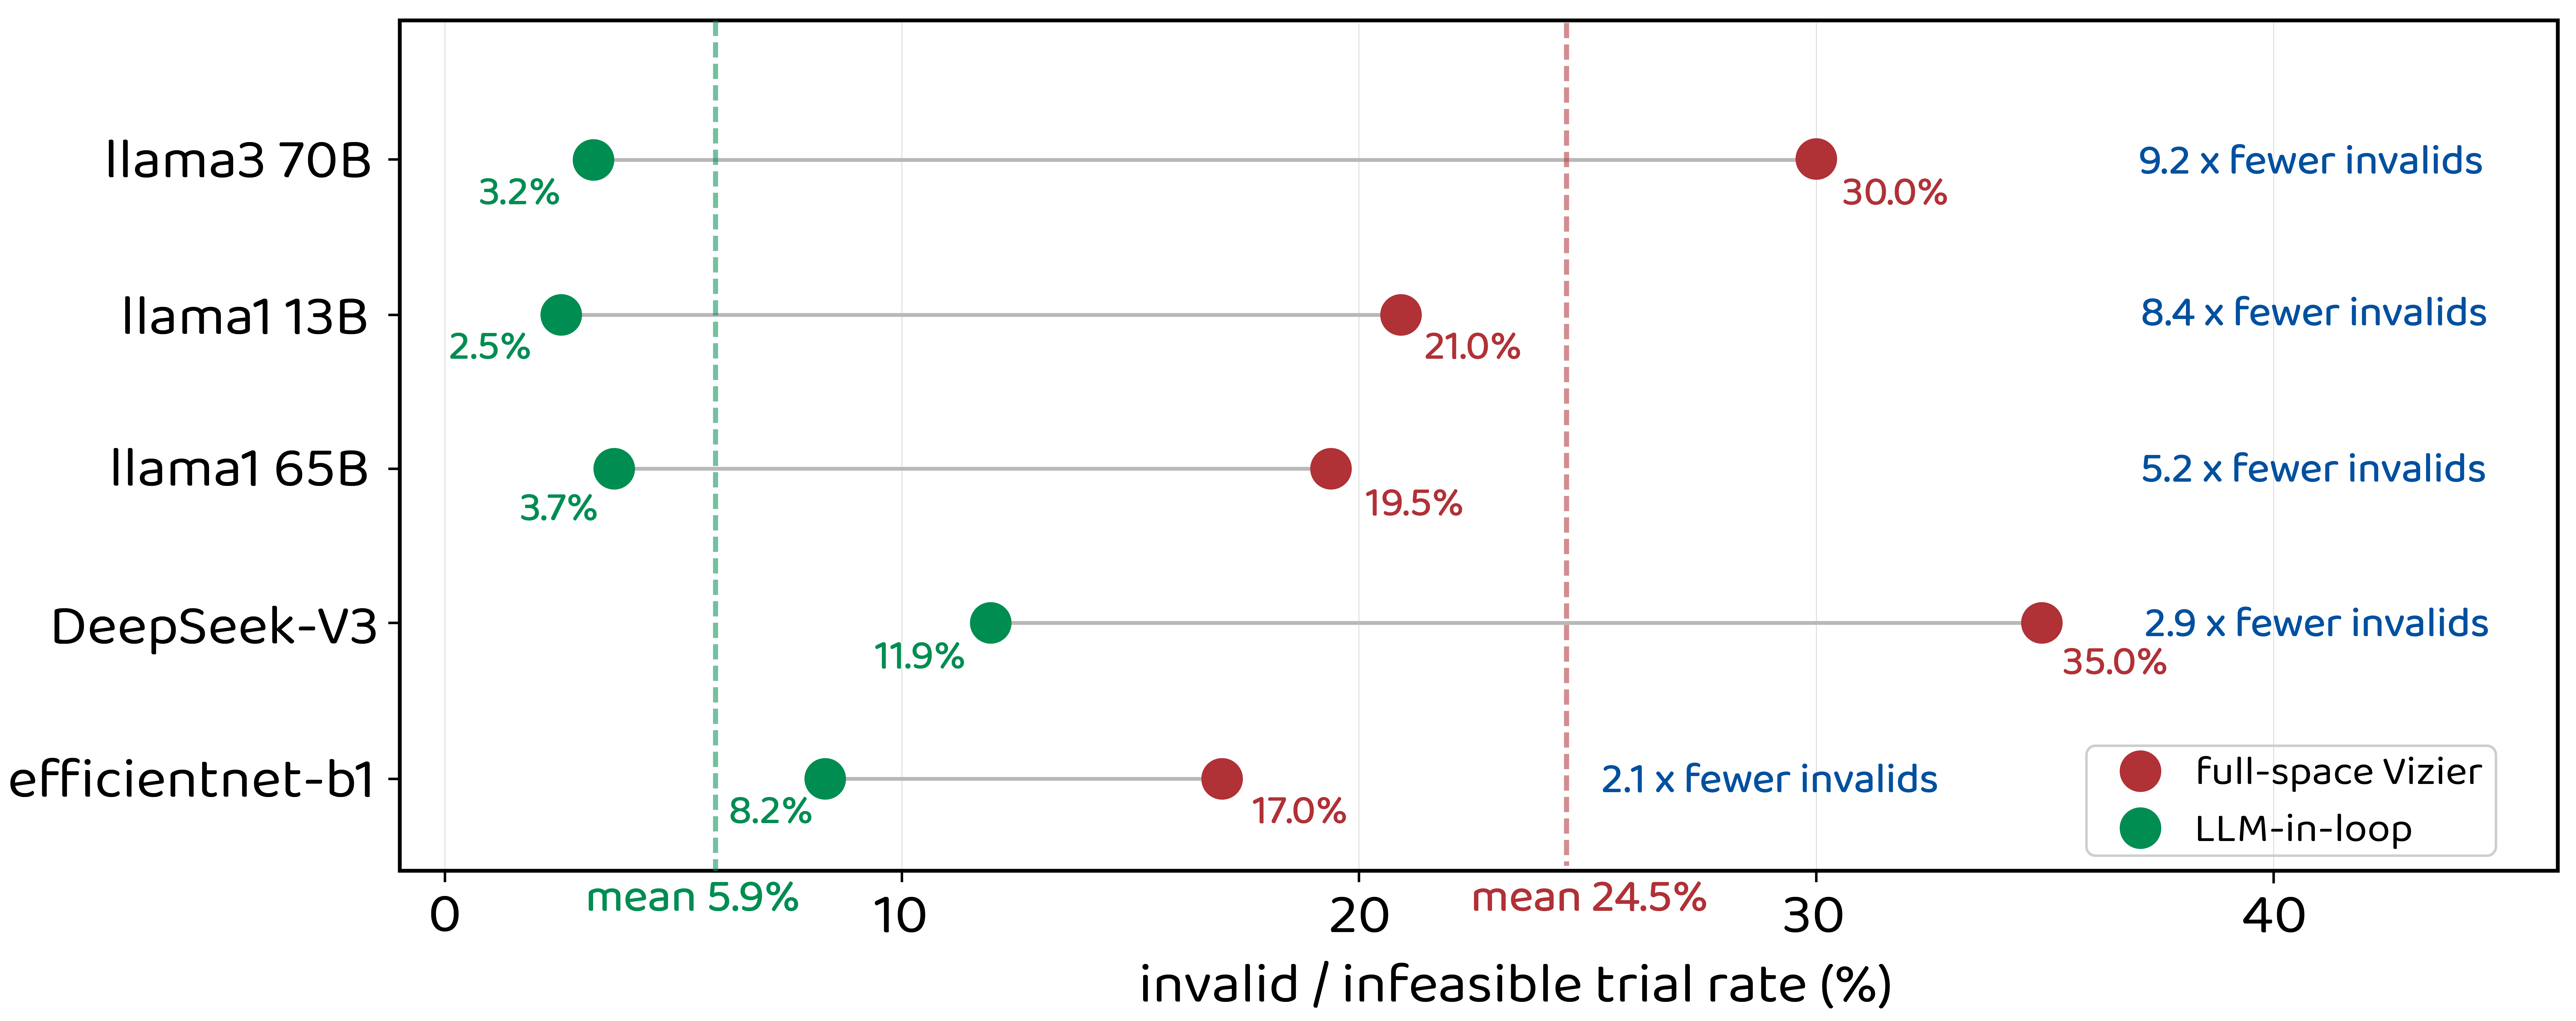
\includegraphics[width=0.85\linewidth]{fig3/llm_guide_v1.png}
% \caption{Invalid/infeasible trial rate (\%) for full-space Vizier vs.\ LLM-in-loop across five workloads. The LLM Architect reduces the mean invalid rate from 24.5\% to 5.9\% (4.1$\times$ reduction), with the largest gains on LLM workloads where the hardware search space is most prone to infeasible configurations.}\label{fig:llm}
% \end{figure}



% The LLM should not just ask, “What chip has the best Perf/TDP?” We aim to answer the question “Given this user’s workload and deployment goal, what is the architectural region to search for this deployment task?”. Therefore we have the LLM emit profile-conditioned campaigns that take specific user inference tasks into consideration. For each $(\text{deployment profile},\ \text{workload})$ cell, we ran a
% 200-trial LLM-Architect experiment using the same Qwen2.5-7B-Instruct + LoRA with differing user input profiles. At the start of each round, the prompt was assembled from a fixed system
% prompt, the active deployment profile, three few-shot examples, and a per-round user message containing the workload, recent feedback signals, current search bounds, and the causal ledger.
% The Strategist returned a one-line JSON campaign patch, which the
% validator accepted only if it was a strict legal subset of the parent space, satisfied hard rules such as patch-volume $\leq 10\%$, ridgepoint and MAC/BW constraints, and avoided forbidden regions.

% Thus, the experiment isolates whether the profile-conditioned LLM prompt alone can steer the same V1 evaluator toward different hardware families under different deployment intents.



% \todo{Compare convergence rate of LLM-guided hardware search vs.\ Vizier-only (Bayesian, LCS, random baselines) in the style of FAST Figure~11. Report:
% \begin{itemize}
%     \item Number of trials to reach $X\%$ of best Perf/TDP found by 5,000-trial Vizier
%     \item Quality of LLM-proposed configurations vs.\ Vizier-proposed configurations
%     \item Qualitative analysis of LLM reasoning about hardware bottlenecks
% \end{itemize}
% }

% \subsubsection{ROI Analysis}

% \todo{Update FAST's ROI analysis (Table~4) with the improved Perf/TDP numbers from FAST-CORGI. Report deployment volumes required to reach 1$\times$, 2$\times$, 4$\times$ ROI targets. If Perf/TDP improvements are larger than FAST's, the break-even deployment volume should decrease correspondingly.}

% \subsubsection{Pareto Frontier}

% \todo{Plot the Perf/TDP vs.\ area Pareto frontier for V1-optimized designs compared to FAST and TPU-v3 baseline, analogous to FAST Figure~12.}